\chapter{连续介质力学} \label{chap2}
\section{引言}
连续介质力学是本文构建控制方程的理论基础。
基于连续介质力学,我们刻画流体以及流体表面,并从两个
视角来描述物体运动,以此构建动力学方程。为了构建完整的控制方程,我们还需要给出本构模型,
即形变与势能的关系,这里我们给出对应的流体的弱可压缩模型以及表面张力模型。

\section{欧拉视角下的动力学}
欧拉视角,即物理量的定义域为$\mathbb{R}^3$,对物体的刻画由空间中的密度场给出。与拉格朗日视角的区别我们将在2.3小节中给出。

\subsection{欧拉视角下的质量守恒定律}
记$\rho : \mathbb{R}^3 \times \mathbb{R} \rightarrow \mathbb{R}$ 为空间中随时间变化的密度场,
$v : \mathbb{R}^3 \times \mathbb{R} \rightarrow \mathbb{R}^3$ 为空间中随时间变化的速度场,此处默认向量为列向量。
\begin{figure}[htbp]
    \centering
    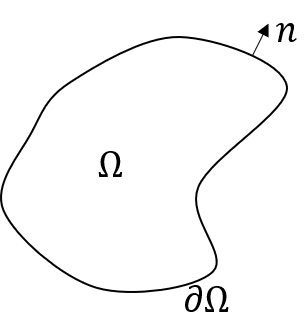
\includegraphics[scale=0.5]{./images/image1.png}
    \caption{}
    \label{fig:example}
\end{figure}

现在考虑一个$\mathbb{R}^3$闭区域$\Omega$,$\Omega$的边界记为$\partial \Omega$,边界上的法向记为
$n$(如图2.1)。同时假定$\rho$ 和 $v$在 $\Omega \times (t_0 - \epsilon, t_0 + \epsilon)$的一个开邻域内足够光滑。根据质量守恒,我们有$\Omega$上质量的
变化率为$\partial \Omega$上质量的流出率和流入率之和。即
\begin{equation}
    \begin{split}
        \frac{d}{dt} \Big |_{t = t_0}\int_{\Omega} \rho(x,t)dx &= -\int_{\partial \Omega} \rho(x,t_0) v(x,t_0) \cdot n(x) ds \\
        \int_{\Omega} \frac{\partial}{\partial t}\Big |_{t = t_0} \rho (x,t)dx &= -\int_{\partial \Omega} div(\rho(x,t_0) v(x,t_0))dx\nonumber\\
    \end{split}
\end{equation}

由于$\Omega$的任意性,由上式可以得到

\begin{equation}
    \frac{\partial}{\partial t}\Big |_{t = t_0}\rho(x,t) + div(\rho v) = 0
\end{equation}

\subsection{欧拉视角下的动量守恒定律}
现在考虑闭区域$\Omega$上的动量变化。根据连续介质力学中的牛顿运动定律[**],闭区域$\Omega$上的动量变化可以分为三部分,
第一部分为物质流入流出$\Omega$导致的动量变化,第二部分为作用在$\Omega$边界上的力导致的动量变化,第三部分为作用在$\Omega$内部物质上的力(一般为重力)产生的作用变化。
即
\begin{equation}
    \frac{d}{dt} \Big |_{t = t_0} \int_{\Omega} \rho v dx = -\int_{\partial \Omega} \rho v (v\cdot n) ds + \int_{\partial \Omega} \sigma \cdot n ds + \int_{\Omega} \rho g dx 
\end{equation}
在(2.2)式中,$g$为重力加速度,$\sigma$为柯西应力[**]。特别的,$\sigma$是一个三阶对称矩阵,其对称性来源于角动量守恒[**],我们将在2.4节中从另一个角度说明其对称性。

由于(2.2)式中$\Omega$选择的任意性,我们有
\begin{equation}
    \frac{\partial}{\partial t} \Big |_{t = t_0}(\rho v) = -div(\rho v^{T}v) + div(\sigma) + \rho g
\end{equation}

矩阵函数散度$div$定义如下:
$$div(A)_i := \sum_j \partial_j A_{ij}$$

(2.2)式变形为
\begin{equation}
    \frac{\partial}{\partial t} \Big |_{t = t_0}(\rho v) + div(\rho v^{T}v) = div(\sigma) + \rho g
\end{equation}


\section{拉格朗日视角下的动力学}
 在上一节中,我们根据质量守恒和动量守恒得到了两个方程(方程(2.1)与方程(2.4)),非常重要的一点是,上述方程并没有使用任何
 有关自然状态--材料在不施加外力的静止状态--的信息。在之后的章节中,我们将假定,$t=0$是处于自然状态,并且只考虑$t \ge 0$ 的情况。

 假定在自然状态下($t = 0$),材料占据的空间为$\Omega_0 \subset \mathbb{R}^3$,此时也称$\Omega_0$为参考构型。对于任意给定的$t\in (0,+\infty)$,
 此时材料占据的空间为$\Omega_t \subset \mathbb{R}^3$,相对于参考构型$\Omega_0$,称$\Omega_t$为当前构型。

 拉格朗日视角和欧拉视角的区别主要是函数的定义域。在上一节中,我们所有函数的定义域都在$\mathbb{R}^3$上,而本节我们将把视角限制在材料上,即
\section{弱可压缩流体}
\section{表面张力}

